%%
%% Beuth Hochschule für Technik --  
%%
%% Kapitel 3 - Android App
%%
%%	

\chapter{Android App}
\section{Android}
Das Betriebssystem ist komplett in der Sprache Java programmiert worden. Dabei handelt es sich um ein Open Source Betriebssystem, welches von der Firma Google entwickelt worden ist. Kern des Betriebssystems ist ein angepasster Linux-Kernel 2.6. 
\subsection{Struktur und Aufbau der App}

\begin{figure}[h]
  \begin{center}
    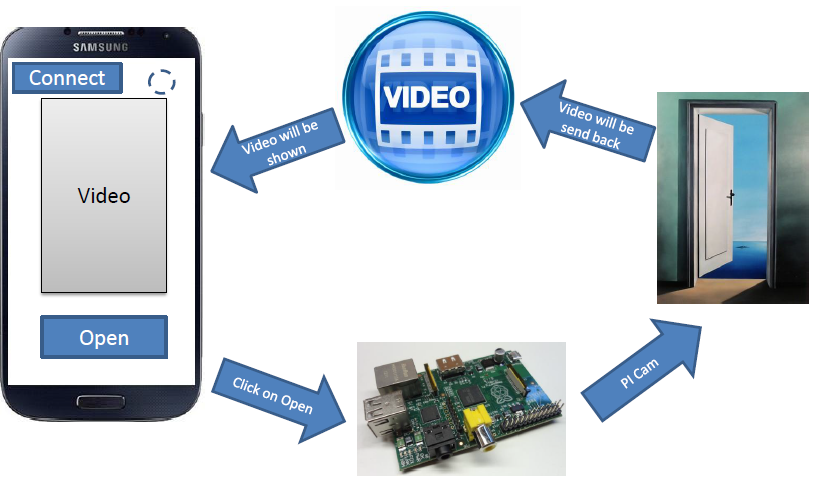
\includegraphics[scale=0.3]{process.png}
  		  \caption{Prozess der App}
     \label{fig.Prozess}
  \end{center}
\end{figure}
Sobald die Control-View geladen ist verbindet sich das mobile Endgerät mit dem Raspberry Pi. Nachdem die Verbindung aufgebaut wurde, kann der Benutzer der App die Schaltfläche \texttt{Open} betätigen. Nach der erfolgreicher Verbindung zum Server sendet dieser einen kontinuierlichen Live-Stream an das Endgerät. Wenn der Benutzter nun die Schaltfläche \texttt{Open} betätigt, wird ein Befehl zum Öffnen der Tür gesendet und ein GPIO angesteuert, der den Türöffner betätigt, um die Tür zu öffnen.

%%%%%%%%%%%%%%%%%%%%%%%%%%%%%%%%%%%%%%%%%%%%%%%%%%%%%%%%%%%%%%%%%%
\subsection{Anmelden des Users}
Um zu verhindern, dass nicht jede Person auf den Stream zugreifen kann, sollte aus Sicherheitsaspekten ein Login implementiert werden. Da aber unerwartete technische Probleme auftraten und diese in der Zeit nicht gelöst werden konnte wurde dieser Aspekt, erst einmal beiseite gestellt.
Jedoch wird im Folgenden auf die Vorgehensweise eingegangen, welche Technologien verwendet worden sind und wie der Login- und Registrierungsprozess ablaufen soll beschrieben.

\subsubsection{Registrierung}
\begin{figure}[h]
  \begin{center}
    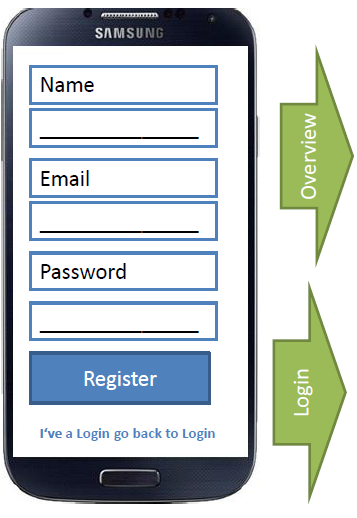
\includegraphics[scale=0.3]{register.png}
  		  \caption{Registrierung}
     \label{fig.Prozess}
  \end{center}
\end{figure}

Um sich überhaupt einloggen zu können muss sich der Benutzer beim aller ersten Mal  mit seinen Kontaktdaten registrieren. Dabei muss der Nutzer seine 
\begin{itemize}
	\item{E-Mail}
	\item{Nutzername}
	\item{Passwort}
\end{itemize}
eingeben.
Das Framework Android-SDK bietet es dem Nutzer an die grafische Oberfläche von der eigentlich Logik zu trennen. Die grafischen Oberflächen werden als Views betitelt. Die Views werden mithilfe von XML gestaltet.
\begin{lstlisting}[caption={Android - Button erstellen},captionpos=b]
<Button
       android:id="@+id/btnLinkToLoginScreen"
       android:layout_width="fill_parent"
       android:layout_height="wrap_content"
       android:layout_marginTop="40dip"
       android:background="@null"
       android:text="Already registred. Log Me In!"
       android:textColor="#21dbd4"
       android:textStyle="bold" />
\end{lstlisting}
In dem obigen Codebeispiel wird ein Button in der View erzeugt. Dabei wird dieser mit einer sog. ID versehen, um den Button über diese ID aus dem Quellcode ansprechen zu können. Mithilfe von \texttt{android:layout\_width} und \texttt{android:layout\_height} wird die Höhe und Breite des Buttons beschrieben. Die Option \texttt{fill\_parent} lässt den Button über die ganze Breite des Bildschirmes anzeigen, abhängig von der Auflösung des Endgerätes. Die Option \texttt{wrap\_content} lässt den Button nur so groß werden, dass alle Inhalte gut zu erkennen sind.
\\
Parallel zu der grafischen Gestaltung der Activity \texttt{Register.xml} wird die eigentliche Logik in Java-Klassen ausgelagert, um eine strikte Trennung von GUI und Fachlogik zu erreichen. Die Klasse \texttt{SignUp.java} ist diesem Fall die Klasse die sich auf das XML-File \texttt{Register.xml} referenziert. Um die einzelnen Objekte des Layouts ansprechen zu können, werden im ersten Schritt alle einzelnen Komponenten erzeugt und im Nachhinein mit der Funktion \texttt{Objekt.findViewByID.ObjektID} auf das jeweilige gerade erzeugte Objekt in der Java-Klasse referenziert.
%%%%%%%%%%%%%%%%%%%%%%%%%%%%%%%
%Code-Beispiel findVIew....
\begin{lstlisting}[caption={Objekt Erzeugung und Referenzierung},captionpos=b]
Button btnRegister;
btnRegister = (Button) findViewById(R.id.btnRegister);
\end{lstlisting}
%%%%%%%%%%%%%
Um überhaupt eine funktionierende Activity zu programmieren brauch man die Funktion \texttt{onCreat()}. In dieser Funktion wird all das ausgeführt was beim starten der Activity passieren soll. Zum einen das Referenzieren auf die erzeugten Objekte und weitere Funktionsaufrufe.
%%%%%%%%%%%%%%%%%%%%%%%%%%%%%%%%
%%Was passiert nun in der Klasse Code und Beschreibung
%%%%%%%%%%%%%%%%%%%%%%%%%%%%%%%%
Diese Daten werden alle in ein JSON-Objekt geschrieben und per POST-Methode an den Server gesendet. Auf dem Server wird in der Index.php erkannt, dass sich ein neuer Nutzer anmelden möchte dem entsprechend wird in einer Mehrfachauswahl (Switch-Case) ausgewertet und in einem weiteren PHP-Skript weiter bearbeitet. Schlussendlich werden die Daten in eine MySQL-Datenbank in die jeweiligen Spalten geschrieben. Das eingegebene Passwort beim Eintragen in die Datenbank verschlüsselt, dass mögliche Hacker die das Password nicht auslesen können. 
\subsubsection{Der eigentliche Login}
\begin{figure}[h]
  \begin{center}
    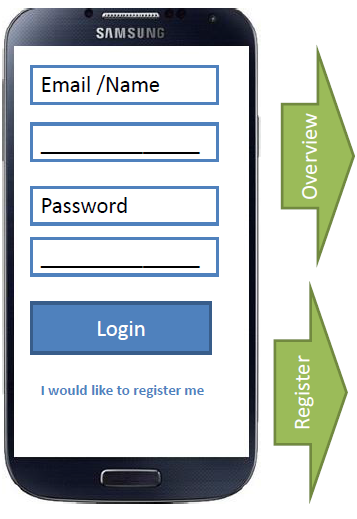
\includegraphics[scale=0.3]{login.png}
  		  \caption{Login}
     \label{fig.Prozess}
  \end{center}
\end{figure}

Beim Login verläuft der Vorgang wie bei der eben beschriebenen Registrierung, bloß in die andere Richtung. Dabei wird ein JSON-Objekt vom Server an das mobile Endgerät geschickt und in der App aufgeschlüsselt und interpretiert. Danach wird verglichen ob sich der Nutzer der sich gerade einloggen möchte schon eingetragen ist, wenn ja wird auf die nächste Activity weitergeleitet, ansonsten wird er zur Registrierung geführt und gebeten sich anzumelden.
\subsection{Control View}
\begin{figure}[h]
  \begin{center}
    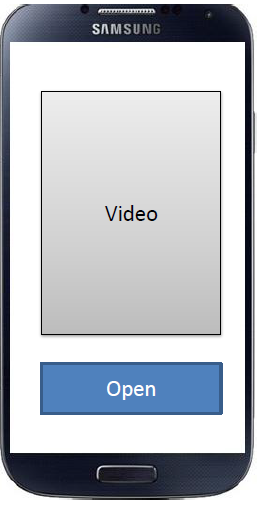
\includegraphics[scale=0.3]{controlcenter.png}
  		  \caption{Control View}
     \label{fig.Prozess}
  \end{center}
\end{figure}
\subsection{Datenbank}
\begin{figure}[h]
  \begin{center}
    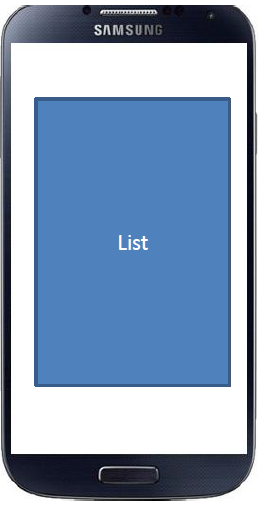
\includegraphics[scale=0.3]{database.png}
  		  \caption{Datenbank}
     \label{fig.Prozess}
  \end{center}
\end{figure}